\documentclass{beamer}

% Use the provided theme
\usepackage{beamerthemetuw}
\usepackage{enumitem}


% Set title, author, date
\title{Rust meets Reality}
\subtitle{Usage, Community and Tooling}
\author{Mark Chimes}
\date{\today}

\begin{document}

% Title slide
\begin{frame}
    \titlepage
\end{frame}

% Outline slide (optional)
%\begin{frame}{Outline}
%    \tableofcontents
%\end{frame}

% Section 1
\section{Rust Tooling} 



\begin{frame}{Licensing} 
Rust Programming Language and official projects dual-licensed:
\begin{itemize}[label=$\bullet$] 
\item
Apache License, Version 2.
\item
MIT license
\end{itemize}
\end{frame} 

\begin{frame}{Rust Tooling and Compilation} 
How does it \emph{feel} to use Rust? 

\begin{itemize} [label=$\bullet$] 
\item Is it easy to get set up? 
\item Is it easy to learn? 
\item Is there good documentation? 
\item Can I figure out when I make a mistake? 
\item Can I find help? 
\item Is the compiler stable?
	\begin{itemize}
	\item
	Bugs: are there many and do they get fixed?  
	\item 
	Will it change out from under me?
	\end{itemize} 
\item Will 
\end{itemize} 
\end{frame} 

\begin{frame}{Basic Tools} 
\begin{block}{}
\begin{tabular}{@{}l l@{}}
\textbf{rustc}        & The compiler \\
\textbf{Cargo}        & Downloads dependencies, compiles packages, 
\\ & makes distributables, and uploads to crates.io \\
\textbf{crates.io}    & Package registry \\
\textbf{rustup}       & Installs toolchain and manages compiler versions \\
\end{tabular}
\end{block}
\end{frame}


\begin{frame}{Standard Tooling} 
\vspace{-3em}
\begin{block}
{Basic functionality included by default}
\begin{itemize} [label=$\bullet$] 
\item compilation \& build files
\item tests
\item dependency \& versioning management
\item documentation generation
\end{itemize}
\end{block}
Compare to Python dependency hell: \\
pip, pip-tools, wheel, pyenv, conda, asdf, venv, virtualenv, pipenv, poetry, pypi, flit, conda-forge, anaconda-repo \ldots
\end{frame} 

\begin{frame}{Getting Started: Running Rustup} 
This installs Rustup, Cargo, the Rust compiler etc. Easy! 
\begin{block}{Linux / Mac}
\texttt{curl --proto `=https' --tlsv1.2 -sSf https://sh.rustup.rs | sh}
\end{block}
\begin{block}{Windows}
Download and run rustup-init.exe (Also requires installing Visual Studio for linker and Windows API)
\end{block}
\end{frame}

\begin{frame}{Example Cargo Commands} 
\begin{block}{}
\begin{tabular}{@{}l l@{}}
\texttt{cargo new}     & Create a new Rust project \\
\texttt{cargo run}     & Build and run \\
\texttt{cargo build}     & Build without running \\
\texttt{cargo test}    & Run tests \\
\texttt{cargo update}  & Update dependencies\\
\texttt{cargo publish} & Publish package to crates.io \\
\end{tabular}
\end{block}

Of course, can use flags 
\begin{block}{}
\texttt{cargo build --release} \hspace{3em} Build optimized version
\end{block}
\end{frame}



\begin{frame}{Compiler Development} 
\begin{itemize} [label=$\bullet$] 
\item
Rust has a very strict stability policy and releases every six weeks. (Run
\texttt{rustup update} to update)
\item
Many features only available on \emph{nightly} toolchain
\item 
Each major decision in Rust starts as Request for Comments (RFC).
\end{itemize} 
\end{frame} 

\begin{frame}{Governance} 

\url{https://github.com/rust-lang/rfcs/blob/master/text/1068-rust-governance.md}
\begin{block}{}
Rust is governed by a core team, [which]:
\begin{itemize} [label=$\bullet$] 
\item    Sets the overall direction and vision for the project;
\item    Sets the priorities and release schedule;
\item    Makes final decisions on RFCs.
\end{itemize}
\end{block}
\end{frame} 




\end{document}


\section{Main Content}



\begin{frame}{Rust in Production - Do You Run Rust Code?} 
\begin{block}{}

\begin{itemize} 
	\item \textbf{Firefox} 
	12\% of code. Migrated server push-notification architecture.
	\item \textbf{Rust-For-Linux Project} 
	Comprises 0.125\% (1/800th) of Linux kernel
	\item \textbf{Ripgrep} 
	Powers text search in VS Code
	\item \textbf{Dropbox}
	components of core file-storage system
	\item \textbf{Cloudflare}
	HTTP proxy (Pingora), DNS stack, DDoS 
	\item \textbf{Git} Added first Rust code a few days ago: 
	libgit-sys and libgit wrappers, and Rust Foreign-Language Interface
	\item \textbf{Ubuntu} plans to replace GNU utilities with Rust implementations
	(e.g. \texttt{ls, cp, find, diff})
\end{itemize} 
\end{block}
\end{frame} 

\begin{frame}{} 
\begin{center}
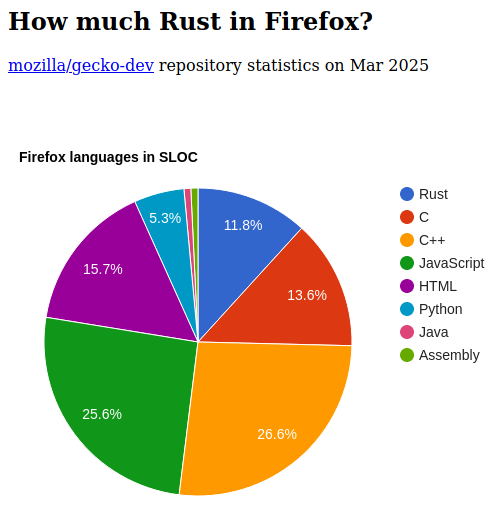
\includegraphics[scale=0.45]{rust-in-firefox}
\end{center}
\url{https://4e6.github.io/firefox-lang-stats/}
\end{frame} 

\begin{frame}{Openhub Rust Language Statistics} 

\begin{center}
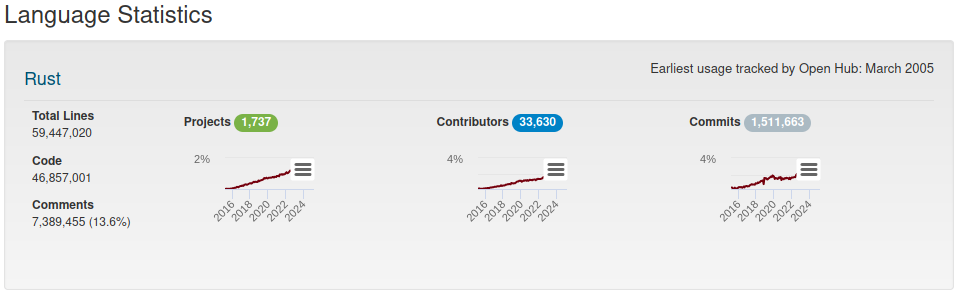
\includegraphics[scale=0.4]{openhub-statistics}
\end{center}

\url{https://openhub.net/languages/rust}


\url{https://madnight.github.io/githut/\#/pull_requests/2024/1}
(next page)

\end{frame} 

\begin{frame}{GitHut 2.0 - Github Language Stats } 
\begin{center}
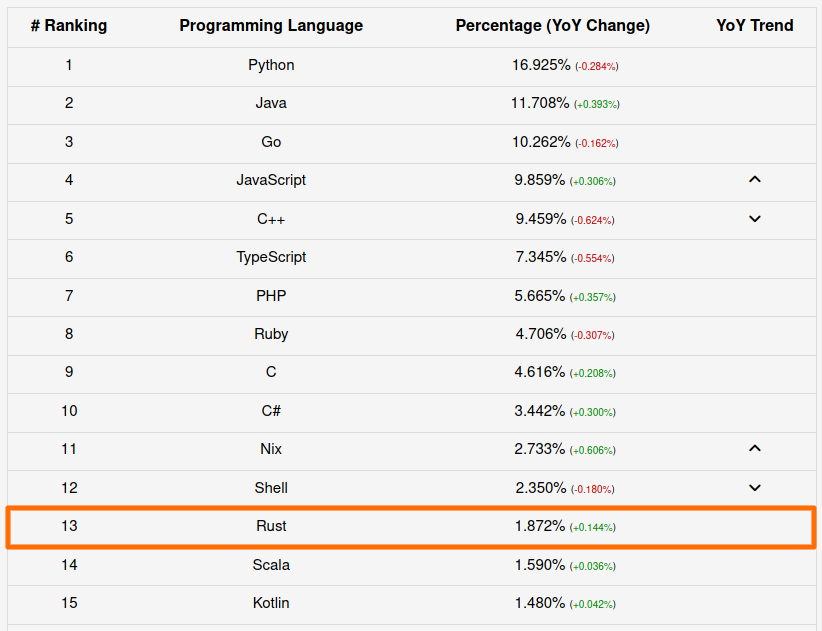
\includegraphics[scale=0.4]{githut-statistics}
\end{center}
\end{frame} 


\begin{frame}{Very Popular With Programmers} 

	\begin{block}{Stack Overflow Survey}

   	Rust is most ``admired", and 6th-most ``desired"

   \end{block}


    \begin{itemize}
    \item \textbf{Admired:} Already use, want to keep using
    \item \textbf{Desired:} Don't use yet, but want to
    \end{itemize} 
    
\end{frame} 

\begin{frame}{Popularity 2023} 
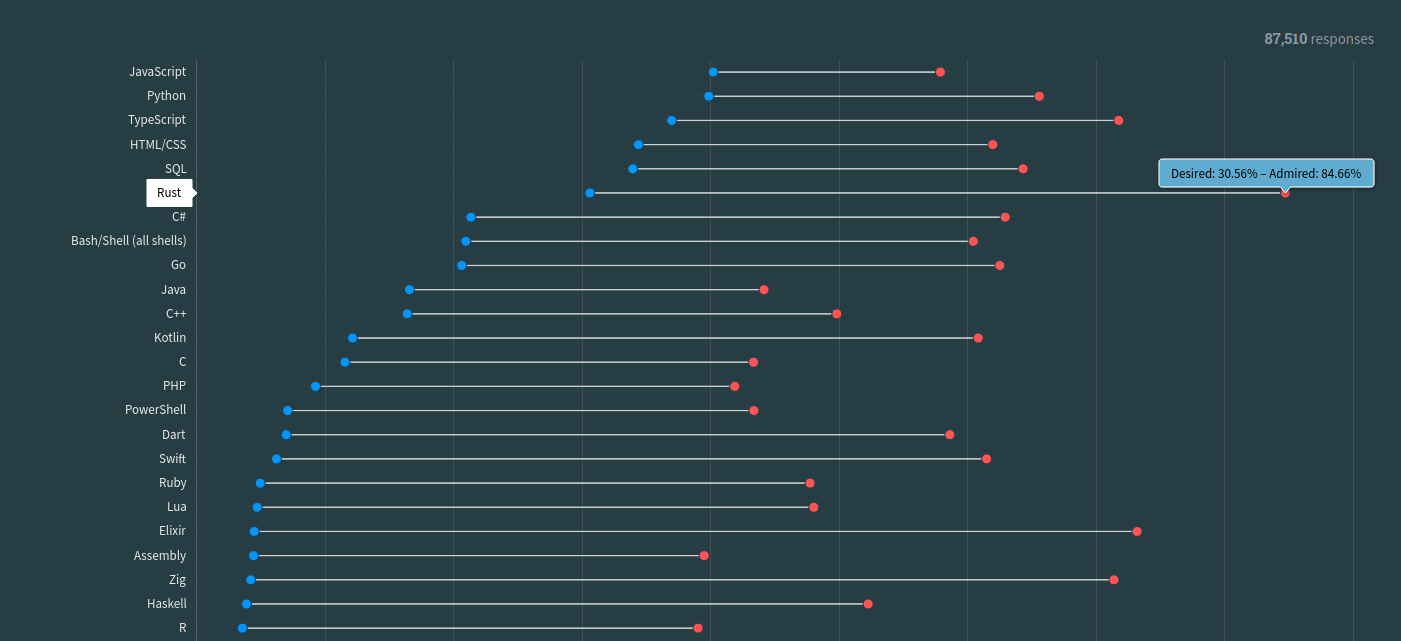
\includegraphics[scale=0.2]{desired-admired-2023}
Admired: 85\%
Desired: 31\%\\
\end{frame} 

\begin{frame}{Popularity 2024} 
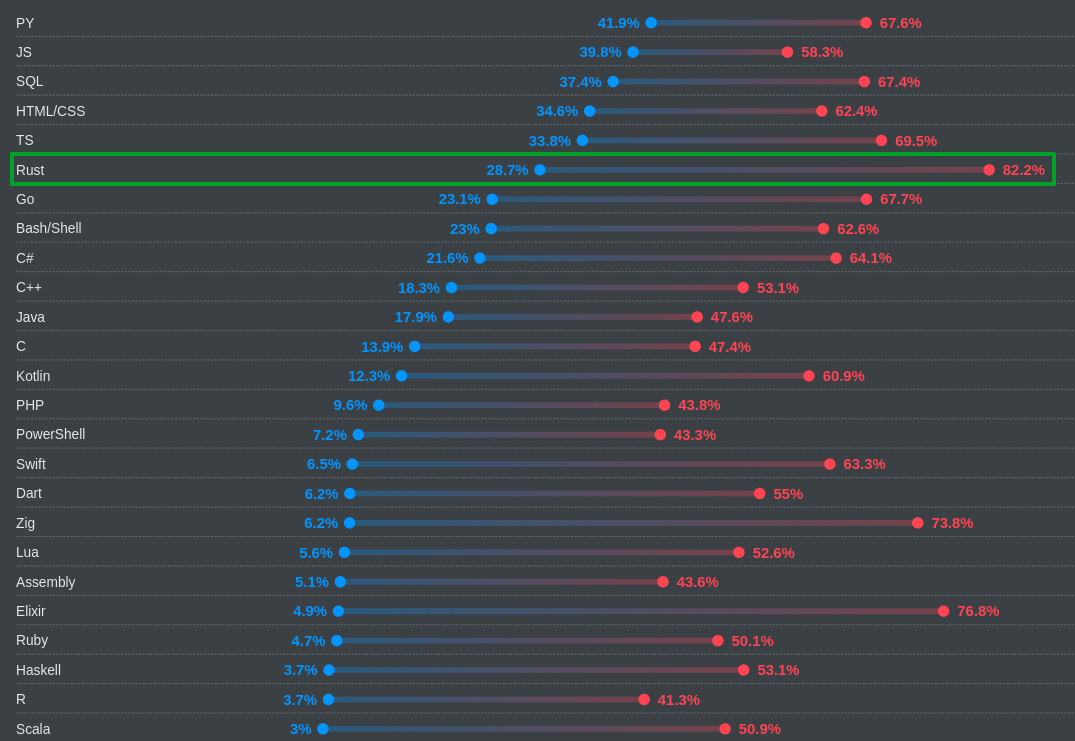
\includegraphics[scale=0.35]{desired-admired-2024}
\end{frame} 

\begin{frame}{History}
    \begin{itemize}
        \item[2006] Personal project by \textbf{Graydon Hoare} working at Mozilla
        \item[2009] Officially sponsored by Mozilla
        \item[2013] Hoare steps down, Rust Core Team formed
        \item[2014] Request for Comments (RFC) process introduced
        \item[2015] Rust 1.0 released
        \item[2016] Rust Mid-Level Intermediate Language (MIR) introduced
        \item[2022] Supported in Linux Kernel
        \item[2024] First Linux (network) drivers written in Rust accepted
	\end{itemize}
\end{frame}

\begin{frame}{Development and Governance} 
\end{frame} 

\begin{frame}{Open-Source and Licensing} 
\end{frame} 


\begin{frame}{title} 
\end{frame} 

\begin{frame}{C and Rust Interop} 
\end{frame} 


\begin{frame}{title} 
\end{frame} 

\end{document}
